{\fontsize{12pt}{22pt} \textbf{Performance metrics for classification}\par}

\vspace{5mm}

1) Accuracy \\

The accuracy is the percentage of correct predictions:

$$accuracy = \frac{1}{n} \sum_{i=1}^{n} \mathbbm{1} \{\hat y_i = y_i \}$$

where $\hat y$ is the prediction and $y$ the true value. \\

\textit{Note}: for imbalanced data, the accuracy can be very misleading because a classifier can achieve a high score just by predicting the majority class with probability 1. \\

In case of binary classification, the accuracy can be written as such: $accuracy = \frac{TP + TN}{TP + TN + FP + FN}$ \\

2) True positive rate \\

The TPR measures the proportions of positives that are correctly identified.

$$TPR = \frac{TP}{P} = \frac{TP}{TP + FN}$$

\textit{Note}: this metric is typically used for medical tasks as it is crucial to minimize the count of false-negatives. \\

3) False positive rate \\

The FPR measures the proportions of negatives that are correctly identified.

$$FPR = \frac{FP}{N} = \frac{FP}{FP + TN}$$

4) ROC (Receiver Operating Characteristic) curve \\

The ROC curve combines the $TPR$ and $FPR$.\\

\underline{Use of the ROC}

\vspace{5mm}

If one model is used:

We use the ROC curve to evaluate the performance of one classifying model that we can obtain when varying a threshold.

\vspace{5mm}

If several models are used:

We use the ROC curve to compare several classifiers in evaluating the area under the curve (AUC) for a range of thresholds.

\vspace{5mm}

\underline{Intuition}

\vspace{5mm}

After running the prediction of a specific model, we draw the confusion matrix (see below) with a certain threshold.

\vspace{5mm}

We then modify the threshold and draw another confusion matrix.

The ROC curve summarizes all of the confusion matrices that each threshold produced.

\vspace{5mm}

\begin{center}
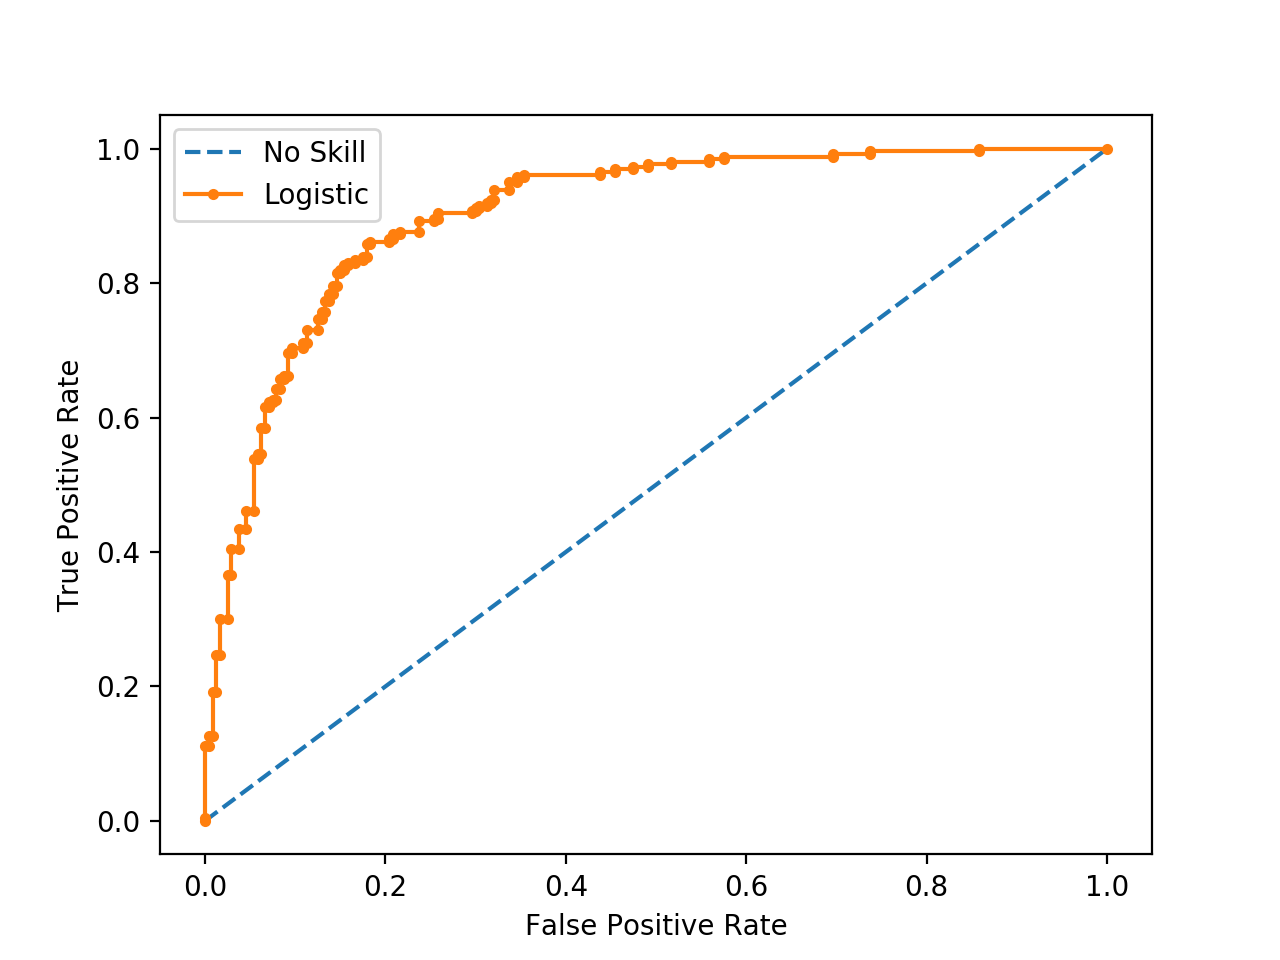
\includegraphics[scale=0.5]{ROC.png}
\end{center}

\vspace{5mm}

\underline{Implementation}

\vspace{5mm}

1. Get probability predictions

2. Sort the probabilities (prediction)

3. Sort the validation (actual) according to previous sort

4. Loop on the sorted validation. At each iteration:

- increment TP or FP

- compute the TPR and FPR.

5. Plot (FPR, TPR)

\vspace{5mm}

See \textit{https://docs.eyesopen.com/toolkits/cookbook/python/plotting/roc.html} for an implementation example, or data challenge Face\_Recognition. \\

5) Precision \\

$$precision = \frac{TP}{TP + FP}$$

\textit{Note}: this metric should be used when false-negative is not too much a concern (e.g. YouTube recommendations). It can also be used when the data are imbalanced (see details below). \\

6) PR (Precision Recall) curve \\

The PR curve combines $TPR$ (recall) and $precision$.

\begin{center}
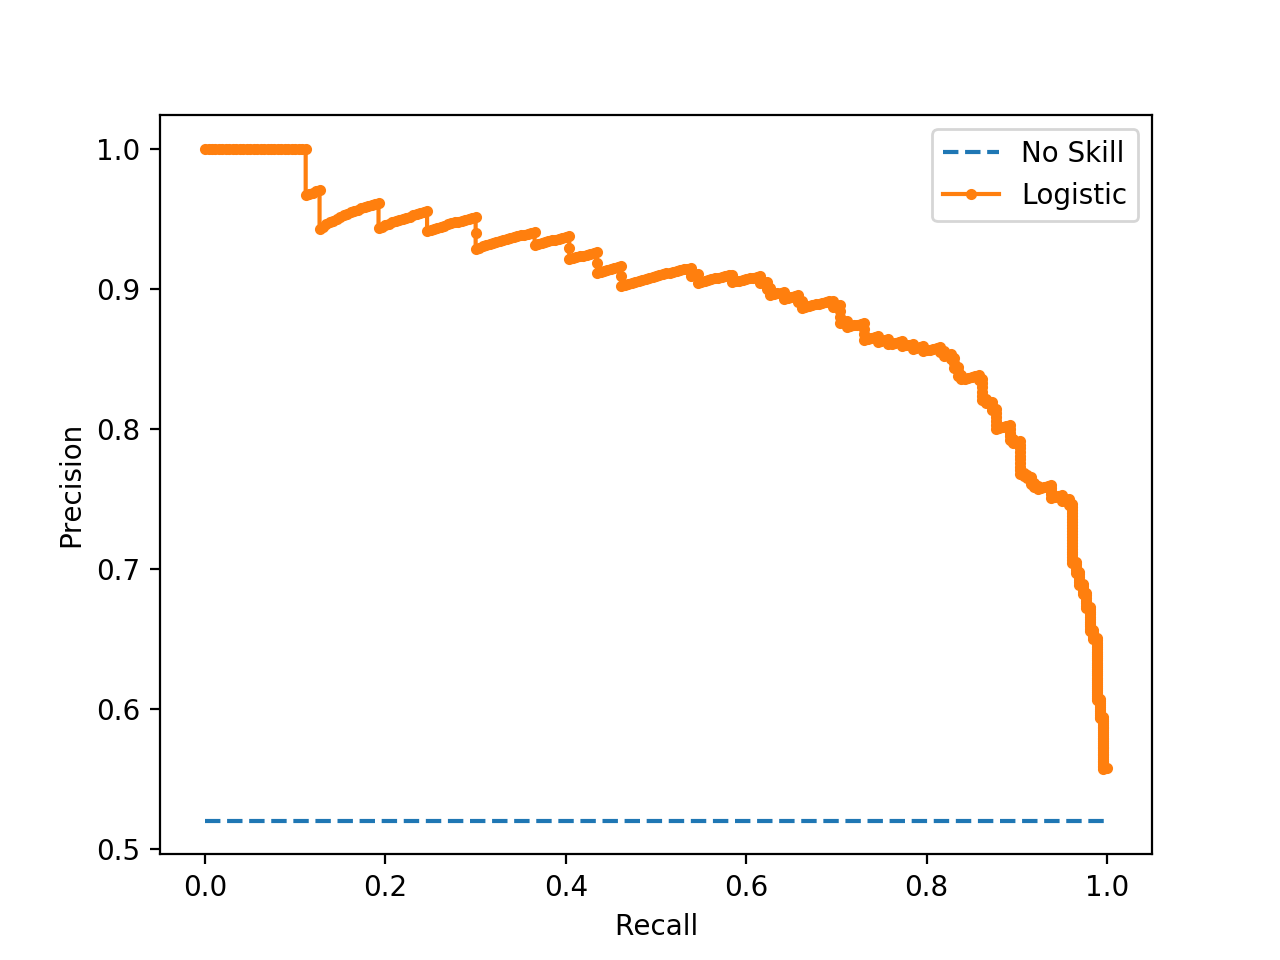
\includegraphics[scale=0.5]{PR_curve.png}
\end{center}

The PR curve is better adapted than the ROC curve in the case of imbalanced data: \\

ROC curve uses $FPR = \frac{FP}{\textcolor{red}{N}} $ --> $N$ can be either very large or very small if classes are imbalanced.

PR curve uses $\text{Precision} = \frac{TP}{\textcolor{green}{TP + FP}}$ --> the precision considers only the positive values coming from the model. \\

7) F1-score \\

F1-score is a single metric that combines TPR (recall) and precision.

$$f1 \text{-} score = 2\frac{precision*TPR}{precision+TPR}$$

\textit{Note}: it is widely used for imbalanced datasets since it involves the precision. \\

\textbf{Metric summary} \\

\begin{center}
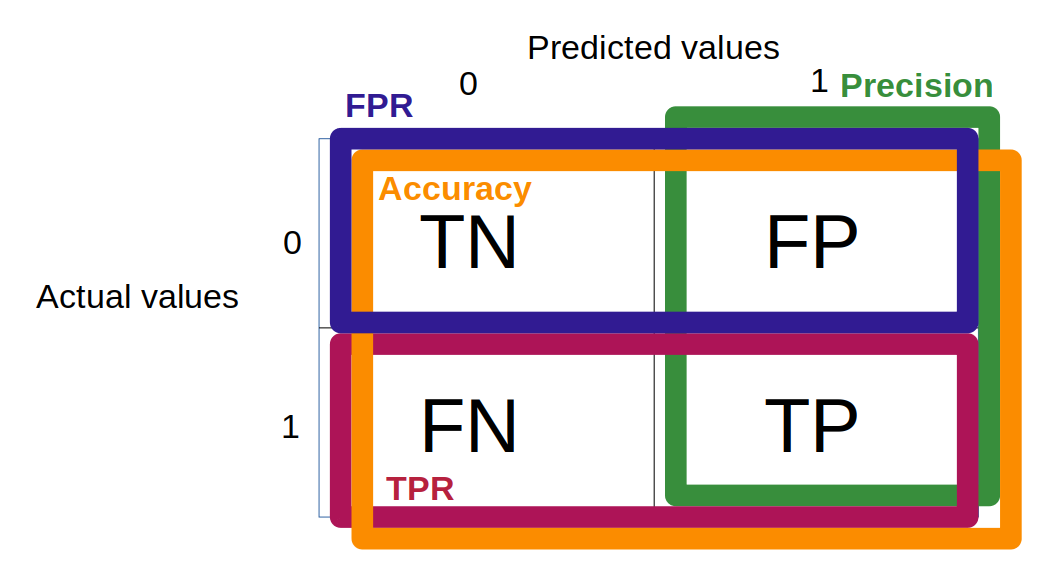
\includegraphics[scale=0.3]{confusion_matrix.png}
\end{center}

\vspace{5mm}
